\documentclass[10pt,a4paper]{article}
\usepackage[english,swedish]{babel}
\usepackage{amsmath}
\usepackage{graphicx}
\usepackage{lmodern}
\usepackage[font=small,format=plain,labelfont=bf,up,textfont=it,up]{caption}
\usepackage[nottoc]{tocbibind}
\usepackage{url}
\usepackage{courier}
\usepackage[T1]{fontenc}
\usepackage[titles]{tocloft}
\usepackage{subfig}

\setcounter{secnumdepth}{5}
\setlength{\parindent}{0in}

\renewcommand{\topfraction}{0.85}
\renewcommand{\textfraction}{0.1}
\renewcommand{\floatpagefraction}{0.75}

\makeatletter
\newcommand\ackname{Acknowledgements}
\if@titlepage
  \newenvironment{acknowledgements}{
      \titlepage
      \null\vfil
      \@beginparpenalty\@lowpenalty
      \begin{center}%
        \bfseries \ackname
        \@endparpenalty\@M
      \end{center}}%
     {\par\vfil\null\endtitlepage}
\else
  \newenvironment{acknowledgements}{
      \if@twocolumn
        \section*{\abstractname}
      \else
        \small
        \begin{center}
          {\bfseries \ackname\vspace{-.5em}\vspace{\z@}}
        \end{center}
        \quotation
      \fi}
      {\if@twocolumn\else\endquotation\fi}
\fi
\makeatother

\title{CuEira, gene-enviroment interaction analysis on GPU}
\author{Daniel Berglund}
\date{March 2014}

\begin{document}
\maketitle

\clearpage
\selectlanguage{english}
\begin{abstract}
Abstract på svenska
\end{abstract}
\clearpage
\selectlanguage{english}
\begin{abstract}
Abstract in english
\end{abstract}
\clearpage
%\begin{acknowledgements}
%Asdf
%\end{acknowledgements}
%\clearpage
\tableofcontents
\newpage

\section{Introduction}
%\subsection{Epidemiology}
%Epidemiology is the study of 

%It combines

%\cite{rothman1998modern,rothman2002intro_epidemiology}

\subsection{Genome-wide association studies}
Genome-wide association studies(GWAS) is a common type of study to search for associations between genetic markers and diseases. Classicaly it doesn't consider interaction between the genetic markers nor enviromental factors. Gene-gene interaction has started to become more common\cite{cordell_detect_review}, however gene-enviroment is still uncommon\cite{gene_enviroment_2013}. Interaction between genes and enviromental factors are considered imporant for complex diseas such as cancer and autoimmune diseases. \cite{cordell_detect_review, gene_enviroment_2013, geira, ra_smoking}\\
\\

These types of studies are usually either cohort or case-control. In cohort studies a sample of a population who don't have the disease is followed. Variables that are suspected to be releveant for the disease is measured and over time some of the individuals will get the disease. The data collected can then be used to find risk factors. In case-control studies two groups are compared to find risk factors. One group consists of individuals with the disease and the other of individuals that are similar to the cases but that doesn't have the disease. \cite{rothman1998modern,mann_observational}\\
\\
The genetic markers are commonly single-nucleotide polymorphisms(SNPs). SNPs are variations in the genome where a single Nucleotide differs between individuals in a population\cite{fareed_snp}. Enviromental factors can be various things such as smoking, physical activity and so on. The amount of data is usually thousands individuals and hundred thousands or millions SNPs. Due to the high number of SNPs few programs investigate more than second order interaction, a few can handle more but not without drawbacks\cite{gwis,high_order_2012,fast_high_order_cluster}.

%Nåt om epistatis här?

\subsection{Defining Interaction}
What do we mean with interaction between factors? There are several definitions of the term\cite{rothman2002intro_epidemiology}. The overall goal is usually to find if \emph{biological} interaction is present. Biological interaction is when the factors co-operate through a physiological or biological mechanism and causes the effect (eg. Disease). This is useful since it's the true interaction in some sense and we can use it to explain the mechanisms involved and possibly find cures for diseas. However it's not well defined, it's not something we can calculate directly from data.\cite{rothman1998modern,rothman2002intro_epidemiology}\\
\\
\emph{Statistic} interaction on the other hand is much more well defined. However it's scale dependant, ie. interactions can appear and disappear based on transformations of the data. It also depends on the model used(eg Logistic, Linear). The common way to define statistic interaction is as the presence of product terms between the factors in the statistical model, this is refred to as \emph{multiplicative} interaction. For instance for a linear model $f(x,y)=ax+by+cxy+d$ c is the product term that implies multiplicative interaction between variables x and y. Statistic interaction is often called just interaction which can make it a  bit confusig.\cite{geira,rothman1998modern}\\
\\
It can also be defined as the divergence from additeve effects

It's called biological interaction by Rothman\cite{} and can also be called \emph{additive} interaction\cite{geira}. Here we we will use the term \emph{causual} interaction.\\

%Something about sufficnt cause?

\subsection{Confounders and Covarietes}
Confounding is one of the central issues in the design of epidemiologic studies. It's when the effect of the exposure is mixed with the effect of another variable. So if we don't measure the second variable the first effect would be estimated as stronger than it really is. The second varialbe is then a \emph{confounder}. Several methods in epidemiology are about avoiding or adjusting for confounding. Sometimes these variables needs to be incorperated into the models. Covarietes are possible confounders or other variables that you want to adjust for in the model. Somtimes covariets are called control variables.\cite{rothman2002intro_epidemiology,rothman1998modern}

\begin{figure}[h]
    \centering
    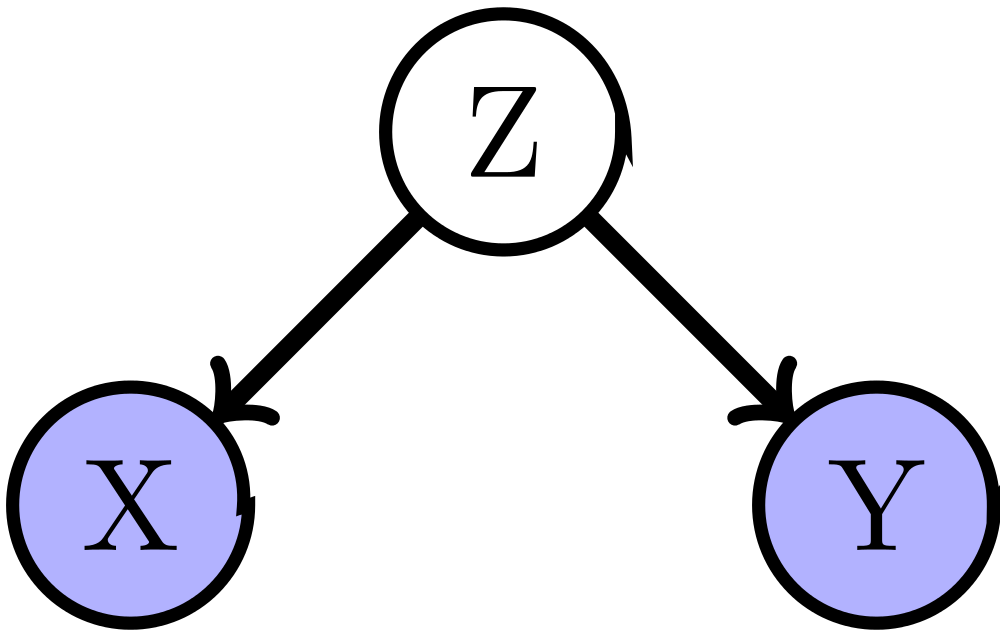
\includegraphics[width=5cm]{Simple_Confounding_Case.png}
    \caption{Illustration of a simple case of confounding. If we don't observe Z we might falesly find an association between X and Y. Wikipedia Commons}
    \label{fig:confunding}
\end{figure}

\subsection{GEIRA and JEIRA}
GEIRA is a tool for analysing gene-gene and gene-enviroment interaction. GEIRA uses additive interaction instead of multiplicative, commonly multiplicative interaction is used\cite{geira}. JEIRA is a parallelized immplementation of the enviromental interaction analysis in GEIRA. However it can only use one node.

\clearpage
\section{Background}
%Mathematical and physical bck (equations etc.)
%Algorithmic bck and concepts (e.g scalability, speedup etc.)
%computer architecture bck(describe CPU and GPU differences etc.)
Most research have focused on gene-gene interaction so there are few tools for gene-enviroment. SNPs are binary variables which is an advantage that is almost always used when searching for gene-gene interaction. They are binary since the three possible combinations of allels(AA, Aa, aa)  can be represtend as 1,1,0 if its dominat model and 0,0,1 if its ressive\cite{}. Enviromental factors can be of any type\cite{gene_enviroment_2013}. Gene-gene interaction tools can sometimes be used to find gene-enviroment interaction, however they usually require the variable to be binary or have other problems since they weren't designed for gene-enviroment interaction. Enviromental factors can also change over time(eg a person can stop smoking, move to a different area) while a persons genome reamains more or less constant.\cite{gene_enviroment_2013}\\
\\
Both CPU clusters\cite{biforce} and GPUs\cite{gwis,gboost,gmdr_gpu,cuda_lr,genie_2012,plink_gpu}, in some cases GPU clusters\cite{} have been used for GWAS. GPUs have been a popular choice since most of the methods for searching for interaction are inherintly good on GPUs because each combination can usually be considered independently from the others. More about this in the section about computer architecture.\\
\\
There are a lot of algorithms and programs proposed for searching for interaction, most have focused on binary variables as already mentioned. They can be rougly classiefed into four categories, exhaustive, stochastic, machine learning/data mining and stepwise\cite{fast_high_order_cluster}. One of the big differences between methods is wether they are testing for interaction or testing for allowing interaction, see section \ref{test_type} for details. In short it's testing if there is interaction or if there might be interaction.\\
\\
Exhaustive search is the most obvious approach, they compare all combinations of the SNPs in the data. They don't risk missing a combination but it also means they can be slow. Multifactor-Dimensionality Reduction(MDR)\cite{mdr_2001} and BOOST\cite{boost_gene_gene} are two examples.\\
\\
Stochastic methods uses random sampling to ``walk'' throught the data. BEAM\cite{beam_2007} is one example and it uses Markov Chain Monte Carlo(MCMC).\\
\\
Machine Learning and Data Mining methods are methods from computer science. They are %TODO
MDR\cite{mdr_2001} is the among the most common methods used in GWAS that is a computer science approach. See section \ref{data_machine_learning} for more details.\\
\\
Stepwise approaches uses a filtering stage and a search stage. At the filtering stage uninterestings combinations are filtered out by using some exhaustive method. The other SNPs are the examined more carefully in the search stage. BOOST\cite{boost_gene_gene} is an example which uses clever datastructures and a likelihood ratio test to filter the data.

\subsection{Contingency Tables}
A contingency table is a matrix used to describe categorical data. Each cell contains the frequency of occurances with a specific combination of variables. Table \ref{table:contingency_table} is an example of an 2 x 3 table. From it we can for instance see that 171 persons that got the placebo had an nonfatal attack. Contingency tables are the basis for various statistical tests to model the data. Contingency tables can be used directly for tests like $chi^2$. \cite{agresti_categorical}

\begin{table}[h]
\begin{tabular}{ l c c c }
  \hline
  & Fatal Attack & Nonfatal Attack & No Attack\\
  \hline
  Placebo & 18 & 171 & 10 845 \\
  Aspirin & 5 & 99 & 10 933 \\
  \hline  
\end{tabular}
\caption{Contingency table describing the outcome of a medical study, from \cite{agresti_categorical}}
\label{table:contingency_table}
\end{table}

\subsubsection{Logisitic and Log-linear Regression}
For logistic regression the cells of the table are Binomial distributed.\cite{agresti_categorical}

In log-linear models Possion distribution is used instead. \cite{agresti_categorical}

\subsubsection{Weighted Logistic Regression}
Need to find the details on this. Each individual is assigned a weight that can be any postive number. It's then used to weight the logistic regression.

\subsubsection{Statistic Measures}
%Nåt om p values?

Relative risk and odds ratio\cite{agresti_categorical}

relative risk due to interaction

AP

Causual bonds

Bonferetti correction

\subsection{Data Mining and Machine Learning Approaches}
\label{data_machine_learning}
Approaches based on Data Mining and Machine Learning have been a popular choice for GWAS. Multifactor-Dimensionality Reduction(MDR)\cite{mdr_2001} and Random Forest(RF)\cite{random_forest} are among the most common\cite{gene_enviroment_2013,cordell_detect_review}. There are others as well such as clustering approaches \cite{fast_high_order_cluster}. Most of them are used for screening the data for possible interactions\cite{gene_enviroment_2013,cordell_detect_review}.\\
\\
Their biggest advantage is that they are usually nonparametric, model free and designed with high dimensional data in mind.
\\
However they are prone to overfitting and the usual way to try to prevent that is to use cross valdiation and sometimes permutation tests. That means that even if the method itself is fast it's repeated so many times that it can be slow in the end\cite{cordell_detect_review}.

\subsubsection{Multifactor-Dimensionality Reduction}
Multifactor-Dimensionality Reduction(MDR) is a method that reduces the number of dimensions by combining several dimensions into one. For GWAS it combines a number of variables from all the variable combinations and its new dimension is then compared against the outcome and if its predictibility is high then the variables that were combined are considred to interact with each other. It goes through all possible combinations of the desired rank like that. It combines the selected n variables by calculating the ratio of cases versus controls for each combination of the possible values of the variables. If the ratio is above a certain threshold all the members of that groups is gets the value 1 for the new dimension, otherwise 0. It's tested with cross valdiation and sometimes permutation tests so it can be slow but is still usually faster than exhaustive search with regression methods.\cite{cordell_detect_review,mdr_2001}\\
\\
%TODO XOR example table

It can been used for gene-enviroment interaction but requires modifications since MDR can only handle binary variables. There are extensions that can use continus variables however they are regression based so they will be slower than regular MDR.\cite{gene_enviroment_2013}

\subsubsection{Random Forest}
Random Forest(RF) is an ensemble learning method, ensemble metods combine multiple models to improve performance. It takes bootstrap samples of the data and builds descion trees on each of them. The trees are then combined to form the classifier. Usually hundres or thousands of trees are used depending on the problem\cite{random_forest}. One of the most popular variants of Random Forest for GWAS is Random Jungle.\cite{random_jungle}
\\
It has been shown in high dimensional data that it tends to only rank interacting factors high if they have strong marginal effects\cite{winham_rf_2012}. Also the ranking of the variables doesn't say which factor it's interacting with either since it's based on the joint distributions\cite{gene_enviroment_2013}. How to incorperate the enviromental factors in RF is also not trivial, using variables with very different scales can bias the results\cite{gene_enviroment_2013}.

%\subsection{Cross Validation, Boosting and Permutation Tests}
%Cross Validation is a common technique for validation in Machine Learning.\\
%\\
%Boosting and Permutation Tests are similar to each other.

\subsection{Test for interaction vs Test for allowing interaction}
\label{test_type}
Test for interaction is the test for the interaction parameter equal zero or not. Aka test saturated vs homogenous assocation\cite{boost_gene_gene}.

Test for allowing interaction on the other hand is . Aka test saturated vs block independance\cite{boost_gene_gene}.

This means that test for allowing for interaction is faster to use so it's commonly used for screening methods.

\cite{cordell_detect_review}
\clearpage
\subsection{Computer Architecture}
Most computers today use the Von Neuman architecture\cite{}. It was first used in EDVAC which was one of the first stored program computers\cite{von1993first}. Stored programc computers uses electronic memory to store the program instructions\cite{computer_arch_2003}.

\begin{figure}[h]
    \centering
    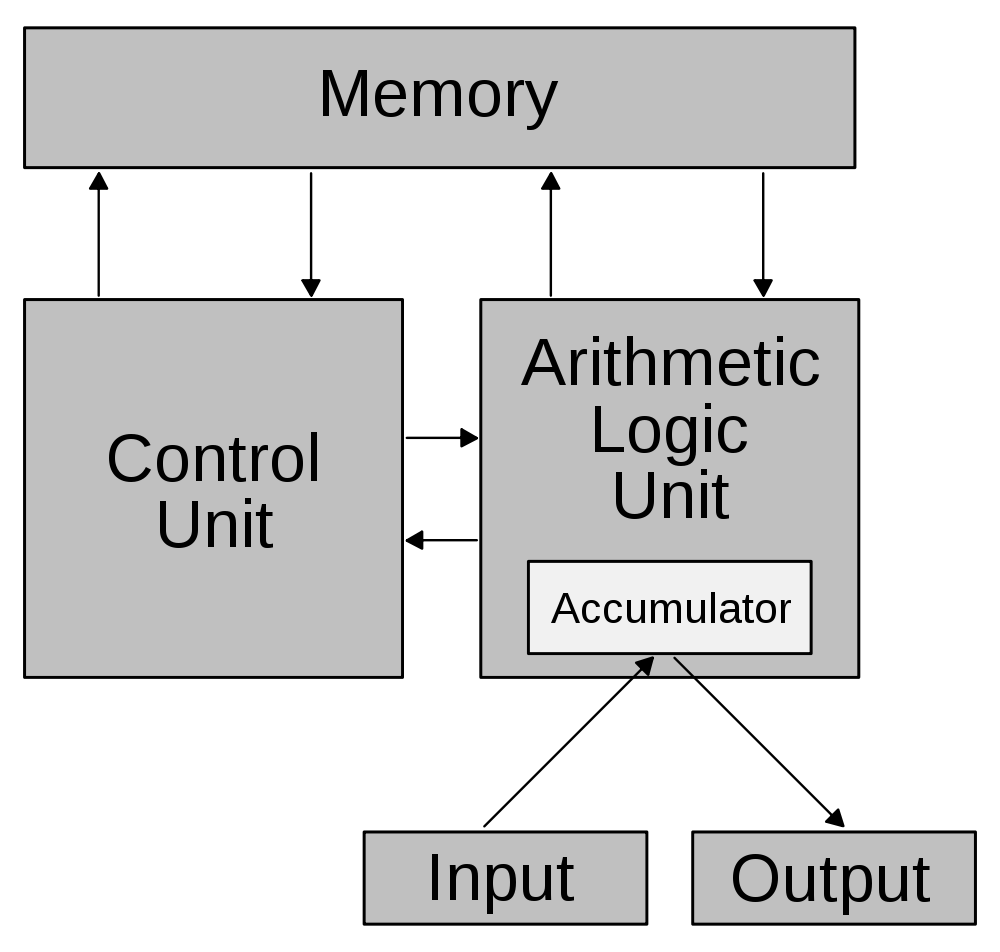
\includegraphics[width=7cm]{Von_Neumann_architecture.png}
    \caption{Schematic of the Von Neuman architecture. Wikipedia Commons}
    \label{fig:VonNeuman}
\end{figure}

\subsubsection{CPU}
Central processing unit(CPU) is 

Until X there was single core CPUs on top 500. Since about 2005 most CPUs have several cores which has increased the need for parallelization. The cores themselves aren't getting faster, the CPUs have more cores.

schematic here

branch prediction
prefetching

\subsubsection{Accelerators, GPU and Xeon Phi}
Graphics processing unit(GPU) have become more popular for general computing the last 10 years.

The table from the cuda guide with performance of GPU vs CPU.\cite{cuda}

something about single and double precision

Xeon Phi

\paragraph{Hetrogenous programming model}
is that

\paragraph{CUDA libraries}
%TODO to have or not to have?
There are several libraries that extend CUDA available.

-cublas
-magma
-thrust
-culatools


%TODO vart ska det här vara?
\subsubsection{Efficient CUDA}
One of the main critizm against GPUs for general computing purposes is that it's hard to get good performance because it requires good knowledge about details of the GPU architecture, especially the memory architecture. There are a few things to keep in minde when writing CUDA programs.\\
\\
assync memory
-streams, conccurent kernels

avoid divergence, aka if statments

avoid bank conflicts

avoid transfers between host and device

minmize divergence

use correct memory
-global
-shared
-constant

textures
-previously imporant, doesn't matter much on modern gpus

\cite{cuda, cuda_best_practice}




\clearpage
\subsection{High Performance Computing}
What is it

More than flops/sec

%Sektioner om i/o, networks etc

\subsubsection{Performance Measures}
An important part in making fast and efficent programs is to know how fast the program is under certain conditions and which parts of the program is slow. For instance the improvment of speed could suddenly drop when we start using to many threads, there might be a bottlneck, and so on.\\
\\
There are two ways to measure how long a program takes to execute. Execution time, sometimes called wall clock time, is how long real life time the program took. The other is to measure the number of processor cycles spent. A parallel program will have shorter execution time than it's serial version however it will likely have spent more processor cycles due to overhead from communcation and initialisation of the threads. We are usually intrested in execution time however number of cycles can be useful for comparasion of algorithms.\\
\\
Speedup is measures how much faster then program is with a certain number of threads compared to the serial version. It's defined as
$$S(p)=T(1)/T(p)$$
Where $T(1)$ is execution time of serial program and $T(p)$ is execution time of parallel program with p threads. Linear speed up is when S(p)=p\\
\\
Efficeny reflects how effcient the program uses p threads. It's defined as
$$E(p)=S(p)/p=T(1)/(pT(p))$$
\\
Amdahls Law is used to find the maximum expected speed up of a system when parts of it won't or can't be parallized. Simply it says that as the number of processors increases the parts that aren't parallized will start taking up more and more of the wall clock time and that the speedup for adding more processors will decrease as more and more processors are added and more time is spent relativly on the non parallized part.\\
\\
The definition is:\\
$$T(p)=T(1)(F+1/p(1-F))$$
Where F is fraction of the code that is serial. The speedup with p threads over 1 thread is then:
$$S(p)=T(1)/T(p)=1/(F+1/p(1-B))$$

\begin{figure}[h]
    \centering
    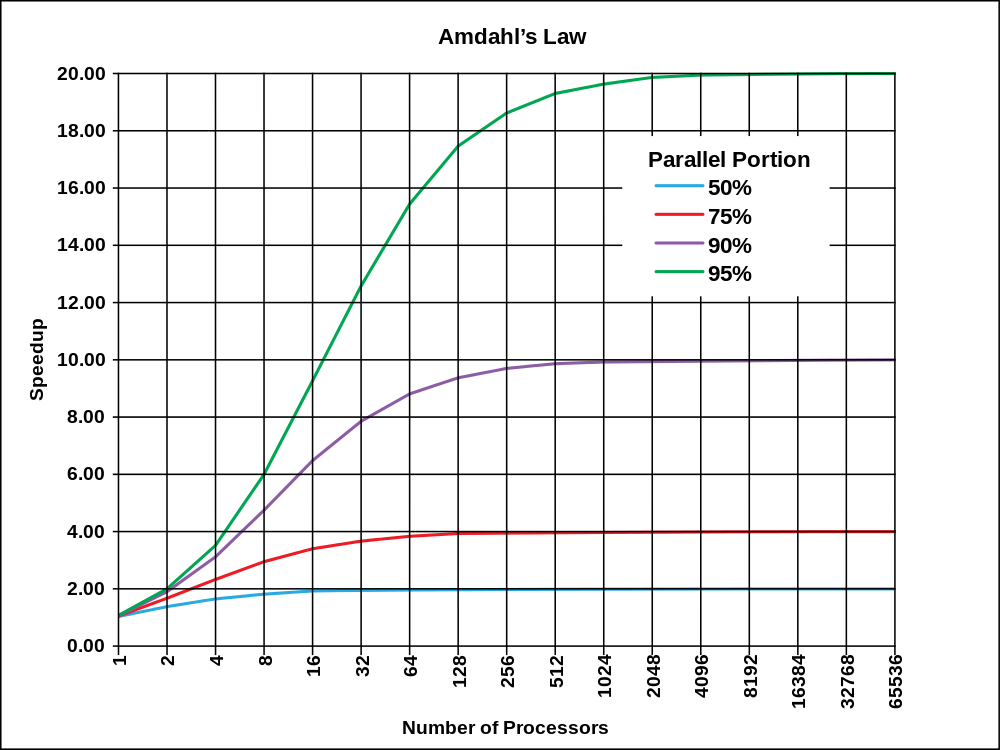
\includegraphics[width=11cm]{AmdahlsLaw.png}
    \caption{Illustration of Amdahls Law. Wikipedia Commons}
    \label{fig:AmdahlsLaw}
\end{figure}

There are limitation to Amdahls Law. BLA BLA

Gustafssons Law

Scalability

Make graphs with number of nodes vs speed, number of cpus vs speed, and so on to show scalability. Also make graphs of data size vs speed to show it handle various data sizes.

\subsubsection{Profilers}
Profilers bla bla

\subsubsection{Clusters}
What are they

Memory spread out etc

Message parsing, pretty much all uses it

Mix of gpus and cpu are common. So the GPUs can do the heavy computation while other parts are used on CPU.

Flops is not everything, bad performace compare to theortical maximum
Stuck in network, harddrives, etc. Latency
Very few programs scale to the fastest clusters, peta scale.

Tianhe 2 is current top. Theoretical performance 54.9 PetaFlops.
Max achived with LinPack 33 PetaFlops
60\% efficiency

\subsection{Which program for GPU and which for CPU?}
This a big question. As with a lot of things it depends on the algorithm to implement etc.

NVIDIA vs Intel performance claims, intel gets much lower than Nvidia. But who can you trust really?

If you have lots of legacy code then then you might need to rewrite a lot. However by using a profiler the parts that take up the most time can be found and moved to the GPU. However that migh be hard if the program isn't properly structured. No legacy code can also be a good thing. Old code might not be written with modern standards or use new nifty features and therefore lose speed.

Xeon Phi is an altnerative

GPUs loses more when going from single precision to double than CPUs. Peak performance on tesla-kepler cards for single precision is around 4 Tflops while double precision is around 1.4 Tflops. \cite{nvtesla}\\ ref the table thing

\section{Algorithm}
%Algorithm (up till 20 pages)
%  - Current state - Basic algorithm, Data structure, memory consumption, parallelization, load balancing and scalability
%  - And the same for own your implementation

%TODO nån typ av intro här

\subsection{Why GPU for GWAS?}
Most approaches to interaction analysis is embarasingly parallel since they consider each combination independtly from the others. That means that those algorithms are likely to work well on GPUs. Several studies got high gains from implementing their programs on GPU, however their CPU versiosn weren't parallelized so it could be that the peformance of the CPU versions could have been improved a lot from CPU parallelization.\cite{gwis,gboost,gmdr_gpu,cuda_lr,genie_2012,plink_gpu}\\
\\
However there have been studies where the authors implemented their algorithm on both CPU clusters and on a GPU. One study needed X cpu nodes to reach the same performance. %cite http://ieeexplore.ieee.org/xpl/freeabs_all.jsp?arnumber=5260739&tag=1&abstractAccess=no&userType=inst

%Exceptions? Possibly stuff like cluster than needs communcation

%OTHERS
%problem with exathsutive

%memory problems(GENIE, CUDALR and so on)

%2 bit 3 bit data storage

%two stage analysis


\subsection{Current algorithm}
JEIRA uses

%Performance analysis

%\subsection{Mine}
%exhaustive and second stage.

%first stage if there is time.

\section{Results}
%Results (up till 15 pages including plots)
%  - Performance measurements (scalability, speedup and efficiency as well as load balancing)
%  - Setup(simulation setup, compilers and hardware setup)
%  - Single node performance
%  - multy-node performance


\section{Discussion and Conclusions}
%Discussion and Conclusions (up to 3 pages)


\section{Outlook}
%Outlook (up to one page)

\section{Appendix}
%List of figs
%List of tables


\newpage
\bibliographystyle{ieeetr}
\bibliography{hpc.bib,statistics.bib,misc.bib}
\end{document}